%%%%%%%%%%%%%%%%%%%%%%%%%%%%% Define Article %%%%%%%%%%%%%%%%%%%%%%%%%%%%%%%%%%
\documentclass{article}
%%%%%%%%%%%%%%%%%%%%%%%%%%%%%%%%%%%%%%%%%%%%%%%%%%%%%%%%%%%%%%%%%%%%%%%%%%%%%%%

%%%%%%%%%%%%%%%%%%%%%%%%%%%%% Using Packages %%%%%%%%%%%%%%%%%%%%%%%%%%%%%%%%%%
\usepackage{listings, xcolor}
\usepackage{parskip}
\usepackage{hyperref}
\usepackage{amsmath}
\usepackage{graphicx}
\usepackage[a4paper, margin = 1.5cm]{geometry}
\usepackage{float}
\usepackage{amssymb}

%%%%%%%%%%%%%%%%%%%%%%%%%%%%%%% Title & Author %%%%%%%%%%%%%%%%%%%%%%%%%%%%%%%%
\title{Use Cases}
\author{Trentin Tommaso}
%%%%%%%%%%%%%%%%%%%%%%%%%%%%%%%%%%%%%%%%%%%%%%%%%%%%%%%%%%%%%%%%%%%%%%%%%%%%%%%

\begin{document}
  \maketitle
  \tableofcontents
  \newpage
  \section{Definizione}
    Diagramma \textbf{comportamentale} modella comportamento esterno del sistema senza specificare come viene realizzato (modella interazione tra sistema e agenti esterni). 
    \begin{itemize}
      \item Può essere usato nella fase di definizione requisiti;
      \item Identifica requisiti funzionali di un sistema;
      \item Descrive in forma sia grafica che (quasi) narrativa le interazioni tra i possibili utenti ed il sistema;
      \item Risponde alla domanda "com'è usato il sistema?";
      \item Viene visto dall'esterno come \textbf{black box} non specificando dettagli interni;
      \item Comportamento del sistma analizzato dal punto di vista dei possibili utenti;
      \item Si presta quindi ad essere compilato a valle di interviste al committente.
    \end{itemize}
    \begin{figure}[h!]
      \begin{center}
        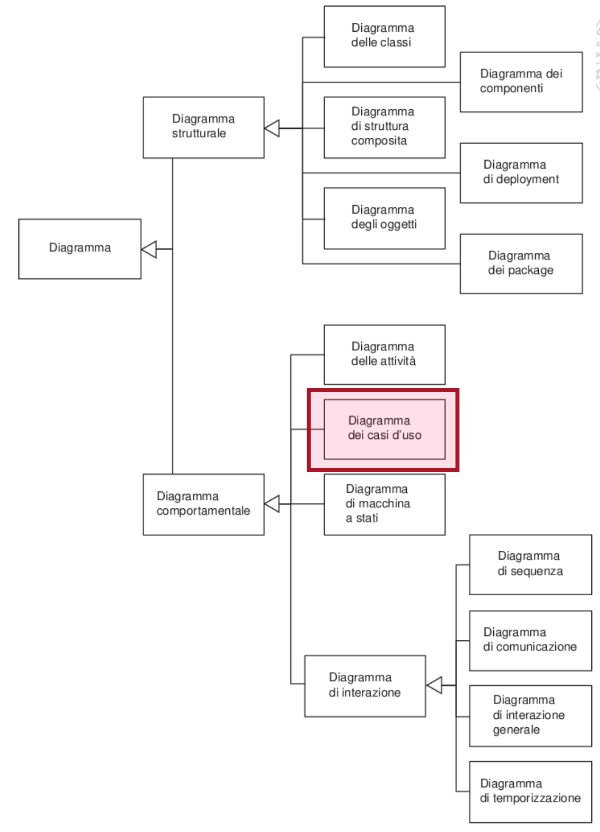
\includegraphics[width=0.5\textwidth]{figures/uml_cu.png}
      \end{center}
    \end{figure}
    \subsection{Scenari e Casi d'uso}
      \begin{itemize}
        \item \textbf{Scenario}: sequenza di passi che caratterizzano una particolare interazione utente / sistema; 
        \item \textbf{Caso d'uso}: insieme di scenari con scopo finale dell'utente in comune;
          \begin{itemize}
            \item Caso d'uso è una tipica interazione tra un attore ed il sistema per svolgere un'attività di lavoro utile; 
            \item Non rivela l'organizzazione interna del sistema;
            \item Insieme dei casi d'uso rappresenta le funzionalità offerte agli attori dal sistema;
            \item Diagramma UML dei casi d'uso spesso comprensibile anche ai "non addetti ai lavori".
          \end{itemize}
        \item I possibili utenti sono \textbf{attori} nello scenario
      \end{itemize}
  \section{Diagramma dei casi d'uso}
    \begin{figure}[h!]
      \begin{center}
        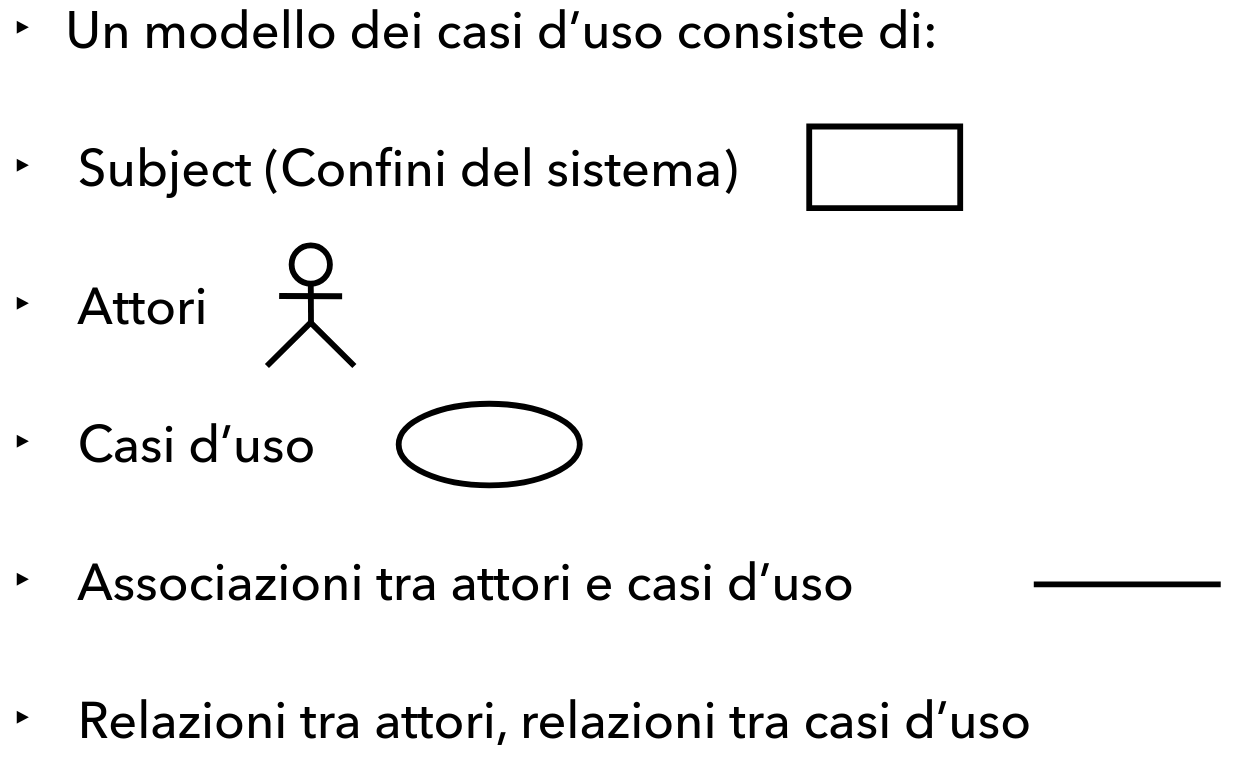
\includegraphics[width=0.5\textwidth]{figures/uml_leg.png}
      \end{center}
    \end{figure}
    \subsection{Subject (confini del sistema)}
      \begin{itemize}
        \item Rappresenta limite tra ciò che è interno al sistema da sviluppare e ciò che è esterno ad esso (è il perimetro che delimita il sistema); 
        \item Rappresentato da un rettangolo etichettato con il nome del sistema;
        \item Ciò che è interno ai confini andrà progettato, realizzato, verificato e validato, costituirà il prodotto SW.
      \end{itemize}
    \subsection{Attore}
      \textbf{Ruolo} (o insieme di ruoli che utente del caso svolge nell'interagire col sistema). Gli attori sono \textbf{esterni} al sistema e possono essere:
      \begin{itemize}
        \item attori \textbf{primari}: perseguono lo scopo che caso d'uso cerca di soddisfare; 
        \item attori \textbf{secondari}: attori con cui sistema interagisce na non interessati allo scopo del caso d'uso.
      \end{itemize}
      Un'attore primario può fornire stimolo che avvia caso d'uso oppure interagisce dopo che caso d'uso è stato avviato.
    \subsection{Caso d'uso}
      Sequenza di azioni che sistema può eseguire interagendo con attori esterni (unità di lavoro utile che sistema esegue dopo a suo innesco). L'innesco viene stimolato dall'attore primario (se esiste) per eseguire compito che attore deve eseguire, oppure può essere effettuato dal sistema, per interagire poi con uno o più attori.
    \subsection{Diagramma}
      Presenta una vista del sistema con attori, casi d'uso (ognuno dei quali può coinvolgere più attori) e loro associazioni. 
      \begin{itemize}
        \item Un attore può partecipare a più casi d'uso; 
        \item Normalmente presenti più clienti, quindi diverse persone potrebbero interpretare attore cliente;
        \item Una stessa persona può ricoprire ruoli diversi e quindi interpretare più attori.
      \end{itemize}
  \section{Descrizione degli Scenari}
    Caso d'uso descritto mediante un insieme di scenari di interazione tra attori ed il sistema, mentre uno scenario è una sequenza di azioni / interazioni fra sistema ed attori. Uno scenario definisce:
    \begin{itemize}
      \item Come / quando inizia caso d'uso; 
      \item Chi inizia caso d'uso; 
      \item Interazione tra attore/i e caso d'uso + ciò che viene scambiato;
      \item Come / quando c'è bisogno di dati memorizzati o di memorizzare dati;
      \item Come / quando caso d'uso termina.
    \end{itemize}
    \subsection{Stili di Descrizione}
      \begin{itemize}
        \item \textbf{Testuali}: flusso chiaro di eventi da seguire; 
        \item \textbf{Diagrammatici}: diagrammi UML di stato, di sequenza, di interazione;
        \item \textbf{Sequenza di passi} numerati: ciascun passo corrisponde a interazione tra attore e sistema, deve essere espresso con una frase semplice che indichi chi lo sta eseguendo e qual è il suo intento senza dettagli tecnici.
      \end{itemize}
    \subsection{Scenari Principali / Alternativi}
      \begin{itemize}
        \item \textbf{Scenario principale di successo}: descrive flusso principale; 
        \item \textbf{Percorsi alternativi}: possono essere di successo o di insuccesso, riportano numero di passo in cui si discosta da scenario principale, condizione da soddisfare per scatenare tale divergenza e, al suo termine, in quale punto rientra nel flusso principale.
      \end{itemize}
    \subsection{Pre e Post Condizioni}
      \begin{itemize}
        \item \textbf{Pre-condizioni}: ciò di cui sistema deve assicurarsi prima di eseguire caso d'uso; 
        \item \textbf{Post-condizioni}: ciò che sistema deve garantire al termine del caso d'uso.
      \end{itemize}
    \subsection{IF, WHILE e FOR negli scenari}
      Cicli WHILE e FOR possono essere usati per racchiudere gruppi di passi da ripetere più volte, le alternative possono essere invece descritte mediante costrutti di delezione IF/ELSE. 
    \subsection{Linee Guida per Descrizione di Scenari}
      \begin{itemize}
        \item Scrivere in stile essenziale senza riferimenti a implementazione; 
        \item Descrivere casi d'uso coincisi e completi;
        \item Descrivere casi d'uso a scatola nera (concentrarsi su responsabilità del sistema e non anticipare scelte alternative);
        \item Nella descrizione di caso d'uso non devono essere indicati dettagli che rivelino scelte di progetto del SW (non vengono affrontati aspetti della progettazione).
        \item Non devono essere presenti riferimenti a specifici file / moduli / interfacce utente, a meno che essi non rappresentino vincoli (es. vincoli dei sistemi già esistenti).
      \end{itemize}
  \section{Relazioni fra Attori e fra Casi d'uso}
    \subsection{Generalizzazione di Attori}
      \begin{itemize}
        \item Attore specialzzato conserva proprietà del generale oltre a possedere sue caratteristiche particolari; 
        \item Freccia parte dall'attore specializzato e punta all'attore generale; 
        \item Generalizzazione tra attori permette di estrarre ruoli comuni a più attori e semplificare diagrammi.
      \end{itemize}
      \begin{figure}[h!]
        \begin{center}
          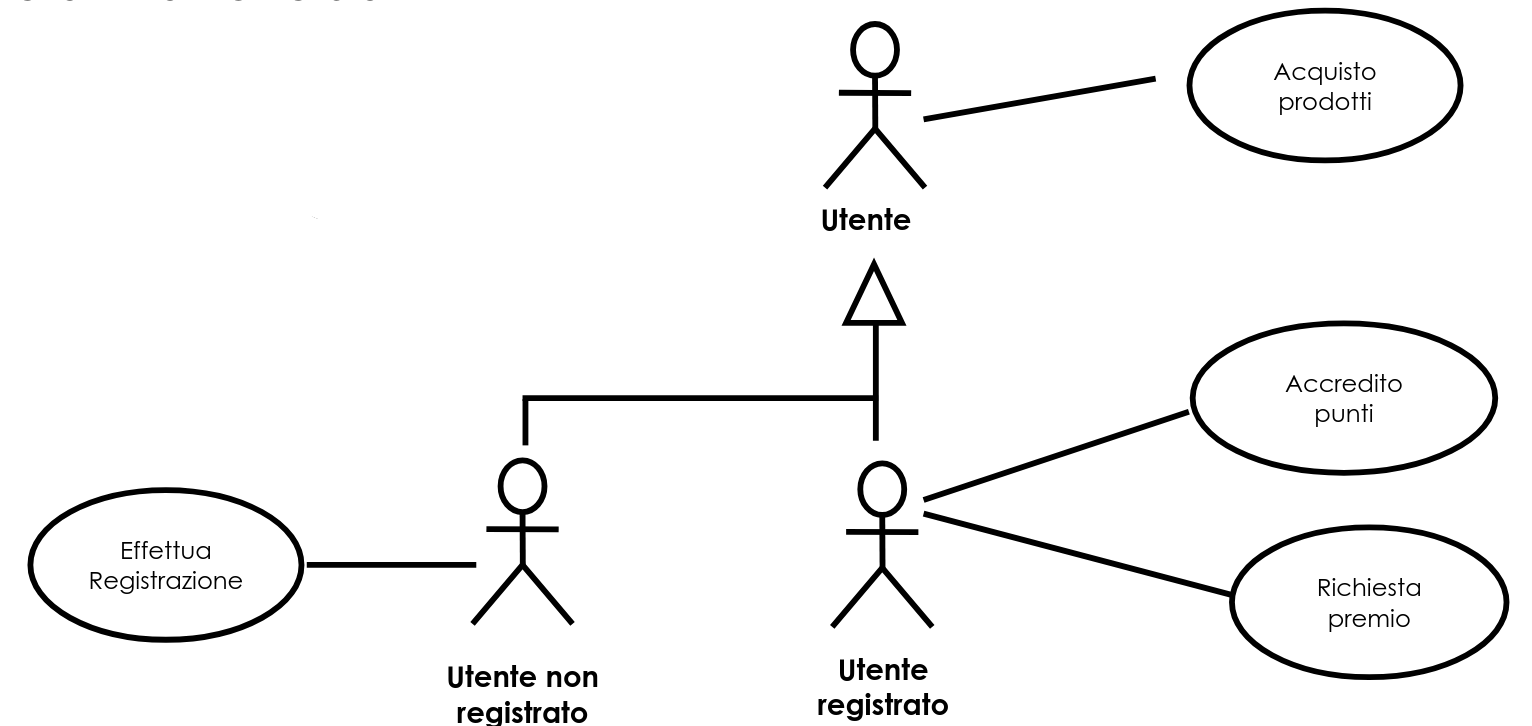
\includegraphics[width=0.5\textwidth]{figures/att_gen.png}
        \end{center}
      \end{figure}
    \subsection{Relazioni fra Casi d'uso}
      \subsubsection{Generalizzazione fra Casi d'uso}
        Simile a generalizzazione fra classi in POO, caso d'uso generale (talvolta astratto) rappresenta diversi casi d'uso simili, mentre uno specializzato eredita comportamento / significato del generale fornendo i dettagli specifici dei casi d'uso simili, può inoltre \textbf{aggiungere passi} o \textbf{modificare il comportamento} del generale. 
        \begin{figure}[h!]
          \begin{center}
            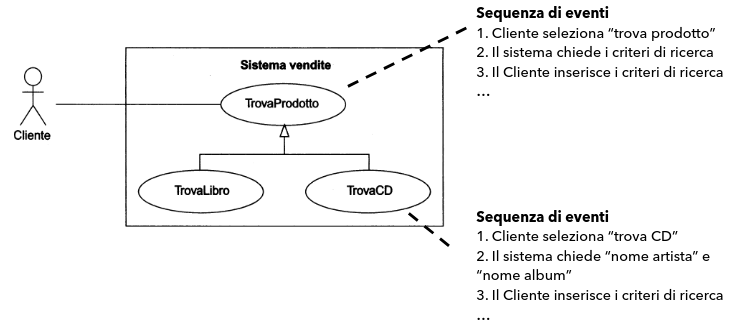
\includegraphics[width=0.5\textwidth]{figures/cu_gen.png}
          \end{center}
        \end{figure}
      \subsubsection{Inclusione fra Casi d'uso}
        Formalizza i casi in cui più casi d'uso \textit{includono} una serie di azioni comuni, ponedo il \textbf{comportamento comune a più casi d'uso} come un caso d'uso incluso nei casi d'uso di partenza. Il caso d'uso base è \textit{incompleto} senza il caso incluso.
        \begin{itemize}
          \item Inclusione non contiene informazioni su ordine dei casi d'uso; 
          \item Caso incluso è una sequenza di azioni eseguita una o più volte dai casi includenti.
        \end{itemize}
        \begin{figure}[h!]
          \begin{center}
            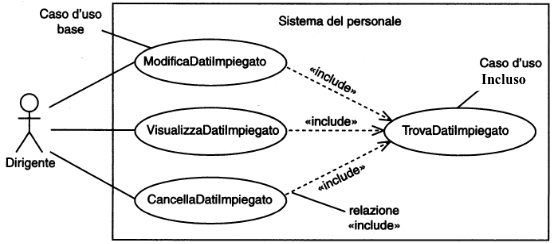
\includegraphics[width=0.5\textwidth]{figures/cu_inc.png}
          \end{center}
        \end{figure}
      \subsubsection{Inclusione e Generalizzazione}
        Se caso d'uso generale include un'altro caso d'uso, tutte le sue specializzazioni "ereditano" tale inclusione. 
        \begin{figure}[h!]
          \begin{center}
            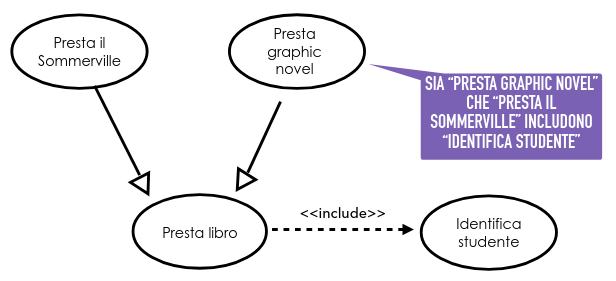
\includegraphics[width=0.5\textwidth]{figures/cu_inc_gen.png}
          \end{center}
        \end{figure}
      \subsubsection{Estensione dei Casi d'uso}
        Modella una sequenza opzionale di eventi / casi eccezionali, ciascuna estensione definisce nuovo caso d'uso che estende caso d'uso di partenza e ne varia comportamento "normale". Nel caso d'uso base si agganciano ad uno o più \textbf{eXtension Points} (XP) le condizioni che fanno scattare l'estensione. 
        \begin{itemize}
          \item Estensione non contiene info su ordine dei casi d'uso;
          \item Estensioni potrebbero anche essere direttamente accessibili da un attore;
          \item In tal caso nel diagramma dei casi d'uso ci sarù una comunicazione (segmento) tra attore e caso d'uso esteso; 
          \item Casi d'uso di estensione aggiungono un comportamento in corrispondenza di XP;
          \item Caso d'uso base si può svolgere anche senza casi d'uso di estensione (a differenza degli include); 
          \item Creando estensioni separate descrizione del caso base rimane semplice. 
        \end{itemize}
        \begin{figure}[h!]
          \begin{center}
            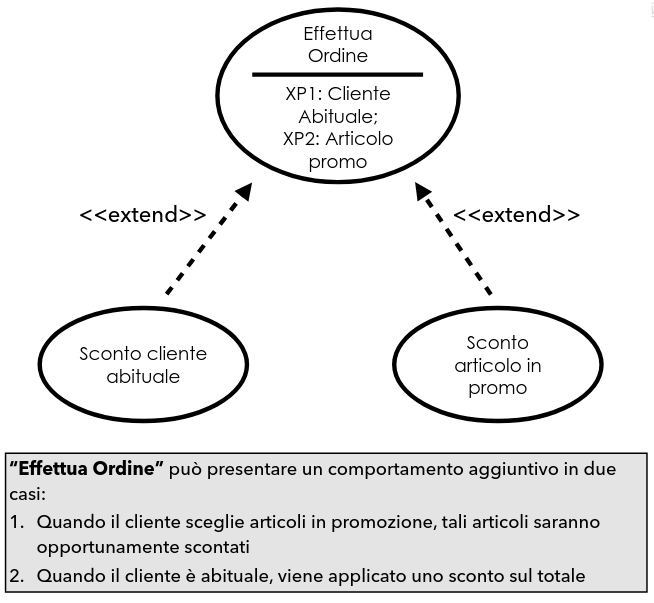
\includegraphics[width=0.5\textwidth]{figures/cu_ext.png}
          \end{center}
        \end{figure}
    \subsection{Errori Tipici con Casi d'uso}
      \begin{itemize}
        \item Dragrammi troppo complessi con molti casi d'uso (ad es. diagrammi di flusso): casi d'uso rappresentano sequenze di azioni, non singole azioni; 
        \item Ripetere nome dello stesso caso d'uso più volte nello stesso diagramma; 
        \item Freccette delle relazioni di estensione o inclusione non sono tratteggiate, oppure nel verso sbagliato:
        \begin{itemize}
          \item <<extend>>: freccia dal caso che descrive evento alternativo al caso base; 
          \item <<include>>: freccia dal caso base al caso che descrive azioni incluse.
        \end{itemize}
      \end{itemize}
    \subsection{Tracciabilità}
      Importante incrociare i requisiti funzionali e i casi d'uso per verificare la reciproca copertura: ogni requisito dev'essere coperto da almeno un caso d'uso e viceversa, tale informazione va riportata nella \textbf{matrice di tracciabiltà}. 
      \begin{figure}[h!]
        \begin{center}
          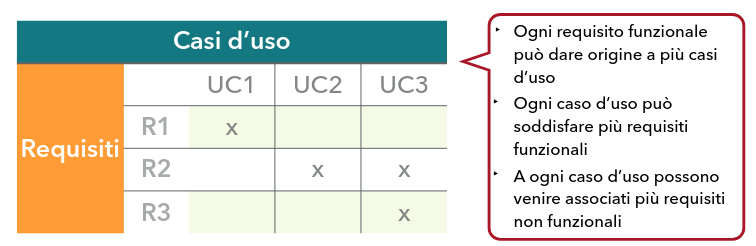
\includegraphics[width=0.5\textwidth]{figures/cu_tra.png}
        \end{center}
      \end{figure}
    \subsection{Prodotto Finale}
      Analisi dei casi d'uso produce un \textbf{diagramma} dei casi d'uso e descrizioni di tutti gli \textbf{scenari} e di tutti i casi d'uso. 
      \begin{itemize}
        \item Nel diagramma viene mantenuto piccolo sottoinsieme delle informazioni contenute nelle descrizioni degli scenari; 
        \item Tutte informazioni contenute nel diagramma sono contenute anche nelle descrizioni degli scenari;
        \item Diagramma dei casi d'uso non dovrebbe mai essere considerato separatamente dalle descrizioni degli scenari.
      \end{itemize}
  \section{Suggerimenti per Costruzione Diagramma Casi d'uso}
\end{document}
